\documentclass[conference]{IEEEtran}
\usepackage{amsmath,amssymb,graphicx,booktabs,tikz}
\DeclareFontShape{OMX}{cmex}{m}{n}{<-> cmex10}{}
\usetikzlibrary{arrows.meta,positioning}
\newcommand{\windRms}{0.119}
\newcommand{\rtkRms}{0.174}
\newcommand{\rtkPeak}{0.685}
\newcommand{\maxTilt}{26.8}
\newcommand{\hoverOn}{0.0000}
\newcommand{\hoverOff}{0.1128}
\newcommand{\poleGood}{-0.582}
\newcommand{\poleBad}{-0.526}
\newcommand{\flightRho}{10}
\newcommand{\dirtyEps}{0.050}
\newcommand{\processA}{0.5}
\newcommand{\processD}{0.3}
\newcommand{\goodCov}{99.98}
\newcommand{\badCov}{99.95}
\newcommand{\goodInnovation}{(+0.000,-0.000,-0.000)}
\newcommand{\badInnovation}{(-0.010,-0.001,+0.015)}
\newcommand{\goodSigma}{0.018}
\newcommand{\badSigma}{0.208}
\newcommand{\meanEstimate}{0.392}
\newcommand{\meanDrag}{0.419}
\newcommand{\ffOn}{0.114}
\newcommand{\ffOff}{0.119}
\newcommand{\driftOne}{0.15}
\newcommand{\driftFive}{1.81}
\newcommand{\driftMaxOne}{0.15}
\newcommand{\driftMaxFive}{1.81}
\newcommand{\tiltNoFix}{43.4}
\newcommand{\dtRatio}{1.000}
\newcommand{\batchId}{full\_20261126\_162018}

\newcommand{\e}{\mathbf e_3}
\newcommand{\rr}{\mathbb R}
\newcommand{\pfig}[2]{\begin{figure}[!ht]\centering
  \includegraphics[width=\columnwidth]{figs/#1.pdf}\caption{#2}\end{figure}}
\tikzset{box/.style={draw,align=center,minimum height=7mm,inner sep=3pt,font=\scriptsize},arr/.style={-{Latex[length=1.6mm]}}}
\begin{document}
\title{Trajectory Tracking of a Quadrotor in Wind\\Sixteen-State LQR and RTK Kalman Navigation}
\author{\IEEEauthorblockN{Aerial Robotics Project 2026}
\IEEEauthorblockA{Aerial Robotics (MSc), Project 2026\\Prof. C. Silvestre}}
\maketitle
\begin{abstract}
This paper designs position and heading tracking for a quadrotor flying
an inspection mission with take-off, two figure-eight laps, and landing.
The design uses a single sixteen-state linear quadratic regulator at
hover, with position and heading integral action. A velocity
implementation places four limited integrators at the actuator input.
Euler-angle torque mapping retains the full attitude kinematics.
A continuous nine-state Kalman filter estimates position, velocity, and
unmodelled acceleration from commanded thrust, measured attitude, and
RTK GNSS position. Two steady-state gains accommodate fixed and degraded
GNSS accuracy. The controller and observer are evaluated together by
linearizing the complete output-feedback dynamics at hover and then
running the nonlinear model with nominal conditions, gusts, loss of
the RTK fix, and vehicle uncertainty with input delay. In estimated
feedback, three-dimensional tracking RMS is \windRms~m in wind and
\rtkRms~m with a five-second degraded fix. The propagated covariance
quantifies the associated increase in position uncertainty. Paired
constant-wind hover tests isolate the steady offset removed by integral
action, and separate trials quantify the performance of disturbance
feed-forward and the drift during complete GNSS loss.
\end{abstract}

\section{Introduction and Notation}
The inspection mission couples thrust, attitude and translation.
The vehicle tracks a prescribed path while navigating with inertial
attitude and RTK GNSS. The implementation follows the supplied
Simulink architecture and the velocity algorithm of Kaminer
\emph{et al.} \cite{kaminer}. Ideal-state runs provide matched
comparisons with estimated feedback.

The inertial frame is North, East, Down (NED).
\(R(\eta)\) maps body to inertial coordinates with ZYX Euler
angles \(\eta=[\phi,\theta,\psi]^\top\) and body rates \(\omega\).
\(\e=[0,0,1]^\top\) and \(S(a)b=a\times b\).
Stars, hats and the subscript \(\mathrm{ff}\) indicate reference,
estimate and feed-forward quantities. Units are SI.

\section{Problem Statement}
\subsection{Nonlinear vehicle and wind}
The plant integrates \(x_p=[p;v;\eta;\omega]\in\rr^{12}\)
from rest at the origin:
\begin{align}
\dot p&=v,\\
\dot v&=-\frac{T}{m}R\e+g\e-\frac{k_d}{m}(v-v_w),\\
\dot\eta&=Q(\phi,\theta)\omega,\\
J\dot\omega&=n-\omega\times J\omega .
\end{align}
Thrust acts along \(-R\e\). The true tilt is
\(\gamma=\arccos(\cos\phi\cos\theta)\) and its limit is
\(0.61\) rad. Each gust satisfies
\(\dot\nu=-\nu/\tau+q\), with white-noise spectral intensity
\(2\sigma^2/\tau\) \cite{jazwinski}.
The mean wind is present from \(t=15\) s. Sensors add
band-limited noise to continuous truth, with spectral
intensity \(r=\sigma^2\Delta t\).

\begin{table}[!ht]
\centering
\caption{Vehicle, disturbance and sensor parameters.}
\footnotesize
\begin{tabular}{@{}ll@{}}\toprule
Quantity & Value\\\midrule
\(m,g,k_d\) & \(1.2\) kg, \(9.81\) m/s\(^2\), \(0.25\) N s/m\\
\(\mathrm{diag}(J)\) & \((0.015,0.015,0.026)\) kg m\(^2\)\\
\(T,\ |n_x|,\ |n_y|,\ |n_z|\) & \([0,24]\) N, \(0.5,\ 0.5,\ 0.1\) N m\\
Wind and gusts & \(2\) m/s north, \(\tau=2\) s, \(\sigma=1\) m/s\\
AHRS, 200 Hz & \(0.5^\circ\) standard deviation\\
Gyro, 200 Hz & \(0.01\) rad/s standard deviation\\
GNSS, 50 Hz, RTK & \(0.02\) m horizontal, \(0.04\) m vertical\\
GNSS, 50 Hz, degraded & \(0.5\) m horizontal, \(1.0\) m vertical\\
\bottomrule\end{tabular}
\end{table}

\subsection{Reference}
The vehicle climbs to \(2\) m in \(5\) s and hovers for \(3\) s.
The horizontal figure eight is
\(3[\sin\beta,\sin\beta\cos\beta]^\top\) m.
Two laps advance \(\beta\) from \(0\) to \(4\pi\).
Two \(4\) s quintic phase-rate ramps add \(4\) s in total to
the two \(20\) s cruise periods. The unwrapped heading follows
the tangent through the eight. The second \(3\) s hover blends
heading to zero, followed by \(5\) s descent and \(2\) s hold.
Position is \(C^2\) at the joins and the velocity and acceleration
are analytic derivatives. Reference channels are sampled at
half the RK4 step so each stage reads an exact table sample.

\clearpage
\subsection{Hover linearization}
Let \(e=R_z(\psi)^\top(p-p^\ast)\),
\(\tilde\eta=\eta-\eta_{\mathrm{ff}}\) with wrapped differences,
\(\epsilon=[e;\tilde\psi]\), and \(\dot\xi=\epsilon\).
The state is \(x=[\xi;e;\dot e;\tilde\eta;\dot{\tilde\eta}]
\in\rr^{16}\) and \(u_\ell=[\delta T;n_\ell]\).
Let \(E\) select \([e;\tilde\psi]\) from the final 12 states
and \(G=gS(\e)\). The hover equations are
\begin{align}
A_h&=\begin{bmatrix}
0&I_3&0&0\\0&-(k_d/m)I_3&G&0\\0&0&0&I_3\\0&0&0&0
\end{bmatrix},\\
B_h&=\begin{bmatrix}0&0\\-\e/m&0\\0&0\\0&J^{-1}\end{bmatrix},\\
A&=\begin{bmatrix}0&E\\0&A_h\end{bmatrix},&
B&=\begin{bmatrix}0\\B_h\end{bmatrix}.
\end{align}
Numerical differentiation checks these blocks against the
nonlinear model. The controllability rank is \(16\).

\section{Controller Design}
\subsection{Exact angular dynamics}
From \(R^\top\dot R=S(\omega)\), using \(R=R_zR_yR_x\),
the mapping from Euler rates to body rates is
\begin{equation}
Q^{-1}=\begin{bmatrix}
1&0&-\sin\theta\\
0&\cos\phi&\sin\phi\cos\theta\\
0&-\sin\phi&\cos\phi\cos\theta
\end{bmatrix}.
\end{equation}
Let \(s=\sin\phi,c=\cos\phi,a=\tan\theta,b=\sec\theta\).
Inversion yields \(Q=[1,sa,ca;\ 0,c,-s;\ 0,sb,cb]\)
with singularity at \(\cos\theta=0\). Differentiation gives
\begin{align}
Q_\phi&=\begin{bmatrix}0&ca&-sa\\0&-s&-c\\0&cb&-sb\end{bmatrix},\\
Q_\theta&=\begin{bmatrix}0&sb^2&cb^2\\0&0&0\\0&sab&cab\end{bmatrix}.
\end{align}
The torque and thrust laws are
\begin{align}
n&=JQ^{-1}(\ddot\eta_c-\dot Q\omega)+\omega\times J\omega,\\
T&=\frac{m(g-a_z^\ast)+w_1}{\cos\phi\cos\theta}
\end{align}
in the upright operating range, with
\(\dot Q=Q_\phi\dot\phi+Q_\theta\dot\theta\) and
\(\ddot\eta_c=\ddot\eta_{\mathrm{ff}}+J^{-1}w_{2:4}\).
The teacher reference uses small-angle roll--pitch feed-forward
\(\phi_{\rm ff}=a^\ast_{h,y}/g,\ \theta_{\rm ff}=-a^\ast_{h,x}/g\)
with \(a^\ast_h=R_z(\psi^\ast)^\top a^\ast\).
Final clipping applies the physical actuator limits.

\subsection{Bryson LQR}
The continuous Riccati solution yields
\(K=R_u^{-1}B^\top P_c\) and \(u_\ell=-Kx\) \cite{anderson}.
The respective maximum scales for the five state blocks are
\((0.5,0.5,0.5,\pi/9)\), \((1,1,1)\), \((1,1,1)\),
\((\pi/9,\pi/9,\pi/9)\) and \((1,1,1)\).
With \(s_u=(6,0.5,0.5,0.1)\), the actual weights are
\(Q_c=\mathrm{diag}(s_x^{-2})\) and
\(R_u=\rho\,\mathrm{diag}(s_u^{-2})\).
The lateral chains couple position with the respective roll
or pitch input. The vertical chain is driven by thrust.
The yaw gain includes angle, rate and heading integral.
The flight setting is \(\rho=\flightRho\).

\subsection{Velocity implementation}
Let \(\chi=[\dot e;\dot{\tilde\eta}]\) be the velocity-level
feedback and \(z\) the low-pass state. The D law uses
\begin{align}
\dot z&=(\chi-z)/\varepsilon_d,\qquad u_\ell=w,\\
\dot w&=-K_I\epsilon-K_e\,d e/dt-K_\eta\dot{\tilde\eta}\nonumber\\
&\qquad-[K_{\dot e}\ K_{\dot{\tilde\eta}}]\dot z .
\end{align}
With \(\dot\psi\) from the gyro and Euler mapping,
\begin{align}
d e/dt&=R_z(\psi)^\top(\dot p_{\rm fb}-v^\ast)-\dot\psi S(\e)e,\\
\dot{\tilde\eta}&=Q\omega-\dot\eta_{\rm ff}.
\end{align}
Ideal feedback has \(\dot p_{\rm fb}=v\). Estimated feedback
uses \(\dot{\hat p}\) here and \(\hat v\) in \(\chi\).
The filter uses \(\varepsilon_d=\dirtyEps\) s.
The four input-integrator limits, measured about hover,
are \([-mg;-n_{\max}]\) and \([24-mg;n_{\max}]\).

In the unsaturated ideal-feedback case with exact derivatives,
integration of the differentiated identity gives
\(w+K_I\xi+K_e e+K_\eta\tilde\eta+
[K_{\dot e}\ K_{\dot{\tilde\eta}}]\chi=\mathrm{constant}\).
Initializing at trim sets the constant to zero and recovers
the linear LQR closed loop at each hover heading.
With finite \(\varepsilon_d\), \(z\) replaces \(\chi\)
in the identity, so the implemented poles include these
six additional dynamics.

\begin{figure}[!ht]
\centering
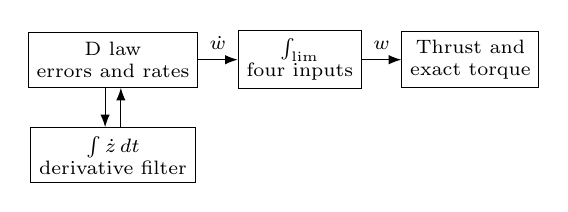
\begin{tikzpicture}[node distance=5mm]
\node[box] (d) {D law\\errors and rates};
\node[box,right=of d] (i) {\(\int_{\rm lim}\)\\four inputs};
\node[box,right=of i] (a) {Thrust and\\exact torque};
\node[box,below=of d] (z) {\(\int\dot z\,dt\)\\derivative filter};
\draw[arr] (d)--node[above,font=\scriptsize]{\(\dot w\)}(i);
\draw[arr] (i)--node[above,font=\scriptsize]{\(w\)}(a);
\draw[arr] ([xshift=-1mm]d.south)--([xshift=-1mm]z.north);
\draw[arr] ([xshift=1mm]z.north)--([xshift=1mm]d.south);
\end{tikzpicture}
\caption{Controller subsystem. The force laws also receive
attitude, rates and the feed-forward reference.}
\end{figure}
\pfig{lqr}{LQR pole locations, selected gain magnitude and normalized
step recovery.}

\clearpage
\section{Estimator Design}
\subsection{Nine-state observer}
The filter predicts \(\ddot p=u_a+d\) with
\(u_a=-T_{\rm cmd}R(\eta_m)\e/m+g\e\).
For \(x_f=[p;v;d]\), the model is
\begin{align}
A_f&=\begin{bmatrix}0&I&0\\0&0&I\\0&0&0\end{bmatrix},&
B_f&=\begin{bmatrix}0\\I\\0\end{bmatrix},&
C_f&=[I\ 0\ 0].
\end{align}
The stacked position observability matrix gives \(I_9\).
Velocity alone gives rank \(6\) and leaves position
offsets unobservable. The correction uses
\begin{equation}
\dot{\hat x}_f=A_f\hat x_f+B_fu_a+L(y-C_f\hat x_f).
\end{equation}
The Riccati gain is \(L=P_\infty C_f^\top R_f^{-1}\)
\cite{kalman}. The process intensity is
\(Q_f=\mathrm{diag}(0_3,q_a^2 I_3,q_d^2 I_3)\), with
\(q_a=\processA,\ q_d=\processD\). The hardware noise fixes
\(R_g=\mathrm{diag}(8,8,32)10^{-6}\) and
\(R_b=\mathrm{diag}(0.005,0.005,0.020)\) in m\(^2\)s.
The status flag selects the healthy or degraded gain.
Complete GNSS loss disables correction.
The first three state equations supply \(\dot{\hat p}\).

\begin{table}[!ht]
\centering
\caption{Flight gain entries. \(K\) indices follow the state order
of Section II. Each filter triplet corresponds to one GNSS axis.}
\resizebox{\columnwidth}{!}{% auto-generated by export_results.m from batch full_20261120_165230 - do not edit
\begin{tabular}{lll}
\toprule
\multicolumn{3}{l}{\textbf{Controller} ($\rho=10$, Bryson scales of Sec.~III):}\\
integrator clamp $\xi_{\max}$ & [0.2, 0.2, 2] m\,s & per-axis anti-windup\\
closed-loop poles $\mathrm{eig}(A\!-\!BK)$ & $\max_t \Re\lambda_t=-0.92$ s$^{-1}$ & slowest decay\\
\multicolumn{3}{l}{\textbf{Estimator} (rw9, $n_x=9$):}\\
drive intensities $(q_a,q_d)$ & (0.5, 0.3) & $Q_9=\mathrm{diag}(0,q_a^2I,q_d^2I)$\\
measurement intensity $R$ & (8.00e-06, 8.00e-06, 3.20e-05) & RTK fix, $r=\sigma^2/f_{\rm rate}$\\
degraded $R_b$ & (5.00e-03, 5.00e-03, 2.00e-02) & fix lost\\
error poles $\mathrm{eig}(A\!-\!L_gC)$ & $\max_t\Re\lambda_t=-0.60$ s$^{-1}$ & RTK-good schedule\\
error poles $\mathrm{eig}(A\!-\!L_bC)$ & $\max_t\Re\lambda_t=-0.60$ s$^{-1}$ & degraded schedule\\
steady-state $1\sigma$ of $\tilde p$ & (0.012, 0.012, 0.021) m & RTK good\\
 & (0.147, 0.147, 0.253) m & degraded\\
\bottomrule
\end{tabular}
}
\end{table}

\newpage
\subsection{Covariance propagation}
With \(D_f=A_f-LC_f\), the predicted error covariance is
\begin{equation}
\dot P_f=D_fP_f+P_fD_f^\top+Q_f+LR_fL^\top.
\end{equation}
It starts at zero because the initialized true and estimated
states agree, including zero disturbance. Both \(L\) and \(R_f\)
follow the recorded fix schedule. Integration on the log grid
gives zero-centered position bands
\(\pm3\sqrt{(P_f)_{ii}}\).
The innovation is \(y-C_f\hat x_f\).

The evaluation residual \(d_{\rm model}\) is actual acceleration
minus commanded-thrust acceleration computed at the true attitude
with nominal mass. True wind drag is reported separately as
\(d_w=-k_d(v-v_w)/m_{\rm true}\).
The residual can therefore include mass and actuation errors.

\subsection{Stability of the coupled dynamics}
The controller and filter use different state models.
Commanded thrust and attitude drive the predictor, and the
disturbance state captures drag and input mismatch tied to
closed-loop motion. The separation theorem for a shared
plant model does not establish stability for this interconnection.
The verified 31-state Jacobian includes the plant, input
integrators, derivative filter and observer.
Its largest real eigenvalue is \(\poleGood\) s\(^{-1}\)
in RTK and \(\poleBad\) s\(^{-1}\) when degraded, over
still-air hover headings \(0,90,180^\circ\).
The uncoupled bonus smoother contributes stable poles at
\(-1\) s\(^{-1}\) with disturbance feed-forward disabled.
The nonlinear trials test switching, actuator limits and delay.

\begin{figure}[!ht]
\centering
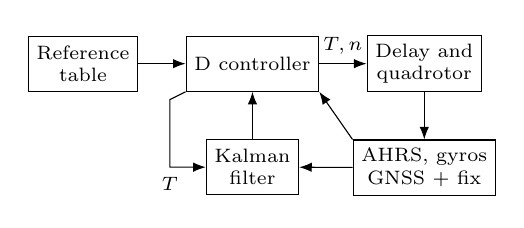
\begin{tikzpicture}[node distance=6mm]
\node[box] (r) {Reference\\table};
\node[box,right=of r] (c) {D controller};
\node[box,right=of c] (p) {Delay and\\quadrotor};
\node[box,below=of p] (s) {AHRS, gyros\\GNSS + fix};
\node[box,below=of c] (k) {Kalman\\filter};
\draw[arr] (r)--(c);\draw[arr] (c)--node[above,font=\scriptsize]{\(T,n\)}(p);
\draw[arr] (p)--(s);\draw[arr] (s)--(k);\draw[arr] (k)--(c);
\draw[arr] (s.north west)--(c.south east);
\draw[arr] (c.south west) -- ++(-2mm,-1mm) |- node[below,font=\scriptsize]{\(T\)} (k.west);
\end{tikzpicture}
\caption{Output-feedback loop. The wind acts on the plant.
The controller also accepts ideal-state feedback.}
\end{figure}

\clearpage
\section{Simulation Setup and Results}
\subsection{Core conditions and metrics}
The \(62\) s mission uses a \texttt{From Workspace} table,
explicit continuous integrators and MATLAB Function blocks.
The solver is fixed-step \texttt{ode4} at \(1\) ms.
Sensors and gusts use paired seeded Band-Limited White Noise
sources. The batch is \texttt{\batchId}.
Each feedback mode is run in still air, mean wind plus gusts,
degraded RTK at \(30\)--\(35\) s, and under two model uncertainty
conditions. Both uncertain runs use \(+20\%\) mass,
\(\pm20\%\) inertia, \(20\) ms actuator delay and wind.

The table compares three-dimensional tracking RMS,
peak error, norm of mean position error in the interior
of the final hover, RMS estimation error in \(p/v/d\), maximum
tilt and control effort. The effort is the RMS norm of
\([(T-mg)/6,n_x/0.5,n_y/0.5,n_z/0.1]\)
from applied inputs after delay.
Estimation-error units are m, m/s and m/s\(^2\).
The estimated-feedback wind run reaches \(\windRms\) m RMS.
The degraded-fix RMS and peak are \(\rtkRms\) and \(\rtkPeak\) m.
Peak tilt across the ten core runs is \(\maxTilt^\circ\).
The 3D animation includes the two vehicle arms, heading, three
trajectories and the horizontal one-sigma covariance ellipse.

\begin{table}[!ht]
\centering
\caption{Paired ideal and estimated mission results.}
\resizebox{\columnwidth}{!}{% auto-generated by export_results.m from batch full_20261119_025000 - do not edit
\begin{tabular}{llrrrrrr}
\toprule
Feedback & Scenario & $E_{\rm RMS}$ [m] & $E_{\max}$ [m] & $\|\mathbf{b}\|$ [m] & est.\ $p$/$v$/$d$ RMS & tilt [$^\circ$] & $U_{\rm RMS}$ \\
\midrule
ideal & nominal & 0.028 & 0.123 & 0.033 & N/A & 15.2 & 0.09 \\
ideal & wind & 0.106 & 0.277 & 0.086 & N/A & 17.1 & 0.11 \\
ideal & rtk lost & 0.106 & 0.277 & 0.086 & N/A & 17.1 & 0.11 \\
ideal & uncert Jplus & 0.113 & 0.391 & 0.082 & N/A & 16.9 & 0.41 \\
ideal & uncert Jminus & 0.113 & 0.391 & 0.079 & N/A & 16.6 & 0.40 \\
estimated & nominal & 0.029 & 0.112 & 0.027 & 0.024/0.16/0.16 & 15.4 & 0.16 \\
estimated & wind & 0.122 & 0.302 & 0.085 & 0.024/0.16/0.31 & 17.4 & 0.18 \\
estimated & rtk lost & 0.208 & 0.958 & 0.085 & 0.106/0.24/0.32 & 32.3 & 0.24 \\
estimated & uncert Jplus & 0.144 & 0.555 & 0.081 & 0.024/0.16/0.50 & 17.0 & 0.45 \\
estimated & uncert Jminus & 0.144 & 0.555 & 0.077 & 0.024/0.16/0.50 & 16.5 & 0.44 \\
\bottomrule
\end{tabular}
}
\end{table}
\pfig{traj3d}{Three-dimensional and top-view trajectories in estimated-feedback wind.}
\pfig{mission_wind}{Reference tracking errors, attitude and applied
wind over the estimated-feedback wind mission.}
\pfig{commands}{Applied thrust and torques for the wind mission.
The thrust reference line is \(mg\).}

\subsection{LQR sweep and integral action}
Table~\ref{tab:rho} compares effort and tracking for all three
weights in paired ideal-state still-air and wind runs.
The time-domain tests use a 1 m position step or a \(10^\circ\)
heading step and report 10--90\% rise, percent overshoot and
2\% settling. Raising \(\rho\) reduces feedback gain along
each controlled chain and moves the closed-loop poles.
The constant-wind hover test ablates the four integral gains.
Mean hover offset over \(35\)--\(45\) s is \(\hoverOn\) m
with integral action and \(\hoverOff\) m without it.
At a feasible unsaturated stationary equilibrium the integral
gain enforces \(\epsilon=0\).

\clearpage
\begin{table}[!ht]
\centering
\caption{Mission weight sweep and normalized step recovery.
Time is in s and overshoot is in percent.}
\label{tab:rho}
\resizebox{\columnwidth}{!}{\begin{tabular}{lrrrr}\toprule
$\rho$ & RMS (still/wind) & Effort (still/wind) & Channel & $t_r$/OS/$t_s$ \\\midrule
0.1 & 0.014/0.078 & 0.090/0.105 & $x$ & 0.65/41.6/4.05 \\
 & & & $y$ & 0.65/41.6/4.05 \\
 & & & $z$ & 0.55/20.8/3.63 \\
 & & & $\psi$ & 0.41/15.4/3.51 \\
1 & 0.015/0.083 & 0.090/0.106 & $x$ & 0.65/42.5/4.07 \\
 & & & $y$ & 0.65/42.5/4.07 \\
 & & & $z$ & 0.58/26.1/3.76 \\
 & & & $\psi$ & 0.49/22.1/3.84 \\
10 & 0.018/0.102 & 0.090/0.106 & $x$ & 0.64/45.3/4.12 \\
 & & & $y$ & 0.64/45.3/4.12 \\
 & & & $z$ & 0.75/34.7/4.19 \\
 & & & $\psi$ & 0.68/30.7/4.25 \\
\bottomrule\end{tabular}
}
\end{table}
\pfig{rho}{RMS trajectory error versus applied-input effort.}
\pfig{hover_int}{Constant-wind hover integral action and ablation.}

\subsection{Estimator tuning and mission validation}
The measurement intensity follows the specified hardware noise.
The process scales allow deviations in the acceleration input
and set the rate at which the disturbance adapts.
The chosen point is evaluated on the degraded-fix transient.

For the degraded-fix mission, aggregate per-axis
\(\pm3\sigma\) coverage across \(p,v,d\) is \(\goodCov\%\)
in RTK and \(\badCov\%\) while degraded.
Innovation mean is \(\goodInnovation\) m in RTK
and \(\badInnovation\) m in the degraded interval.
These are finite-realization estimates from correlated sensor
samples. The horizontal root-sum variance increases from
\(\goodSigma\) to \(\badSigma\) m before re-acquisition.
In the wind-on evaluation window the north mean disturbance
estimate is \(\meanEstimate\) m/s\(^2\), and the mean true
north drag is \(\meanDrag\) m/s\(^2\).
A same-noise half-step check gives the wind RMS ratio
\(\dtRatio\). Two key scenarios are also tested on five
independent holdout seeds.

\pfig{est_err}{Position estimation error with zero-centered
propagated uncertainty bands.}
\pfig{rtk_outage}{Position error and propagated horizontal
uncertainty through five seconds of RTK degradation.}
\pfig{dhat}{Estimated disturbance, model acceleration residual
and physical wind drag.}

\clearpage
\subsection{Bonus trials}
\emph{Disturbance feed-forward.} A unity-DC third-order
smoother filters \(\hat d\). Subtracting the result from the
desired acceleration yields corrections to the roll--pitch
feed-forward and its derivatives in the heading frame.
On the paired estimated-wind run the RMS is \(\ffOn\) m
with feed-forward and \(\ffOff\) m with integral control alone.
The experiment metrics also record effort and tilt.

\emph{Complete GNSS outage.} The estimator predicts without
measurement correction for 1 s and 5 s. The last outage
sample drifts \(\driftOne\) and \(\driftFive\) m respectively,
with window peaks \(\driftMaxOne\) and \(\driftMaxFive\) m.
The maximum tilt across the two full bonus missions is
\(\tiltNoFix^\circ\), above the \(0.61\) rad course limit.
To bridge longer outages, downward
optical flow with altitude sensing would provide an independent
horizontal velocity update. Range or barometric altitude
would also constrain vertical drift.

\pfig{ff}{Paired wind disturbance feed-forward test.}
\pfig{nofix}{Complete GNSS outages and recovery through landing.}
\pfig{holdout}{Independent wind and degraded-fix validation seeds.}

\section{Conclusions}
A 16-state hover LQR yields a velocity-form controller with
four limited actuator-input integrators. The coupled hover
dynamics are stable at both GNSS accuracies tested.
Nonlinear trials compare wind, sensor degradation and delayed
model uncertainty under common error and effort measures.
The hover ablation measures integral action, while covariance
propagation quantifies the change in uncertainty during fix
loss and supports three-dimensional replay.

\begin{thebibliography}{9}
\bibitem{kaminer} I. Kaminer, A. M. Pascoal, P. P. Khargonekar, and
E. E. Coleman, A velocity algorithm for the implementation of
gain-scheduled controllers, \emph{Automatica}, vol. 31, no. 8,
pp. 1185--1191, 1995.
\bibitem{anderson} B. D. O. Anderson and J. B. Moore,
\emph{Optimal Control: Linear Quadratic Methods}. Dover, 2007.
\bibitem{kalman} R. E. Kalman, A new approach to linear filtering
and prediction problems, \emph{J. Basic Eng.}, vol. 82, no. 1,
pp. 35--45, 1960.
\bibitem{jazwinski} A. H. Jazwinski, \emph{Stochastic Processes and
Filtering Theory}. Academic Press, 1970.
\end{thebibliography}
\end{document}
